\documentclass[10pt,pdf,aspectratio=169]{beamer}
\usetheme{CambridgeUS}

\usepackage{graphicx}
\usepackage{subfigure}

\usepackage{caption}
\captionsetup[figure]{labelformat=empty}% redefines the caption setup of the figures environment in the beamer class.

%\setbeamertemplate{caption}{\raggedright\insertcaption\par}

% \usepackage{dsfont}
\usepackage{cancel}
\usepackage[export]{adjustbox}
\usepackage{amsthm}
\usepackage{amsmath}
%\usepackage{stmaryrd}
\usepackage{ulem}
% \usepackage[backend=biber,style=numeric-comp,sorting=none]{biblatex}
\usepackage{stmaryrd}

\usepackage[english]{babel}
\usepackage{fontspec}

%\usepackage{subcaption}
\usepackage[]{graphics}
\usepackage{mathtools}
\usepackage{cite}

%\graphicspath{{../images}}

\setmainfont{cmun}[
  Extension=.otf,
  UprightFont=*rm,
  ItalicFont=*ti,
  BoldFont=*bx,
  BoldItalicFont=*bi,
]
\setsansfont{cmun}[
  Extension=.otf,
  UprightFont=*ss,
  ItalicFont=*si,
  BoldFont=*sx,
  BoldItalicFont=*so,
]
\setmonofont{cmun}[
  Extension=.otf,
  UprightFont=*btl,% light version
  ItalicFont=*bto,%  light version
  BoldFont=*tb,
  BoldItalicFont=*tx,
]

\usepackage{tikz}
\usepackage[beamer]{hf-tikz}
\usepackage{pgfplots}
\usepackage{ragged2e}
\usepackage{bbm}

\usetikzlibrary{arrows,automata,shapes,calc,patterns,arrows.meta}
\usetikzlibrary{fadings}

% \pgfplotsset{
%   axis line style={thick, black!50},
% }
\tikzset{
  every picture/.style={line width=1pt},
  >=latex
}

\makeatother
\title[Перетворення відеозапису з дошки у слайд-шоу]{
  \huge{Перетворення відеозапису з дошки у слайд-шоу}
}

\author[Доповідач: Максим Шило,  Науковий керівник: Водолазський Є. В.]{
Доповідач: Максим Шило\inst{1} \and
Науковий керівник: Водолазський Є. В.\inst{1}}

\institute{
  \inst{1} Національний технічний університет України
  ``Київський політехнічний інститут імені Ігоря Сікорського''}

\date[]{16 червня 2022}

\setbeamertemplate{theorems}[numbered]

\DeclareMathOperator{\argmax}{argmax}
\DeclareMathOperator{\argmin}{argmin}
\DeclareMathOperator{\rank}{rank}

% \bibliographystyle{plain}
% \addbibresource{proofs}
% \bibliography{proofs}

\begin{document}

\begin{frame}
  \titlepage
\end{frame}

\begin{frame}
    \frametitle{Мотивація}
    \begin{figure}
        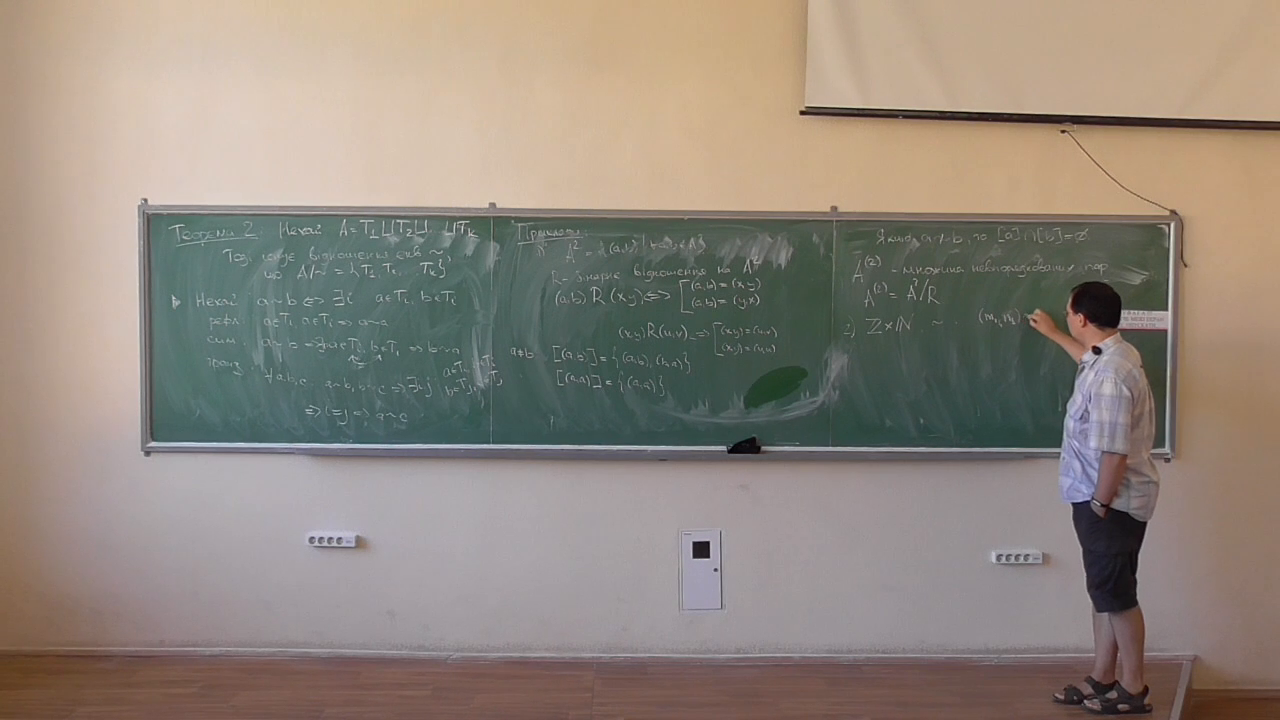
\includegraphics[width=0.4\textwidth]{images/before.png}
    \end{figure}
    \begin{figure}
        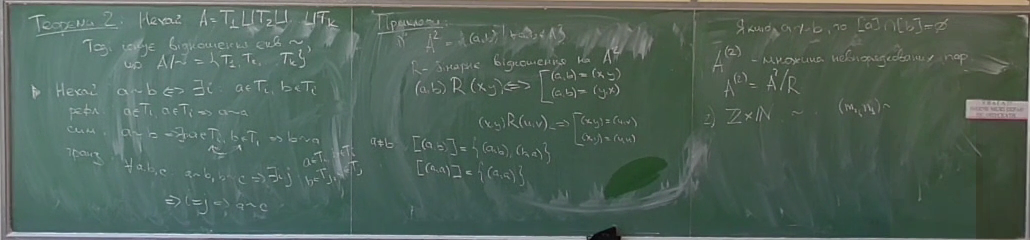
\includegraphics[width=0.7\textwidth]{images/after.png}
        \caption{Джерело ~---~\url{https://youtu.be/a7TUp4p-pIk}
        }
    \end{figure}

\end{frame}

\begin{frame}
    \frametitle{Мотивація}
    \begin{figure}
        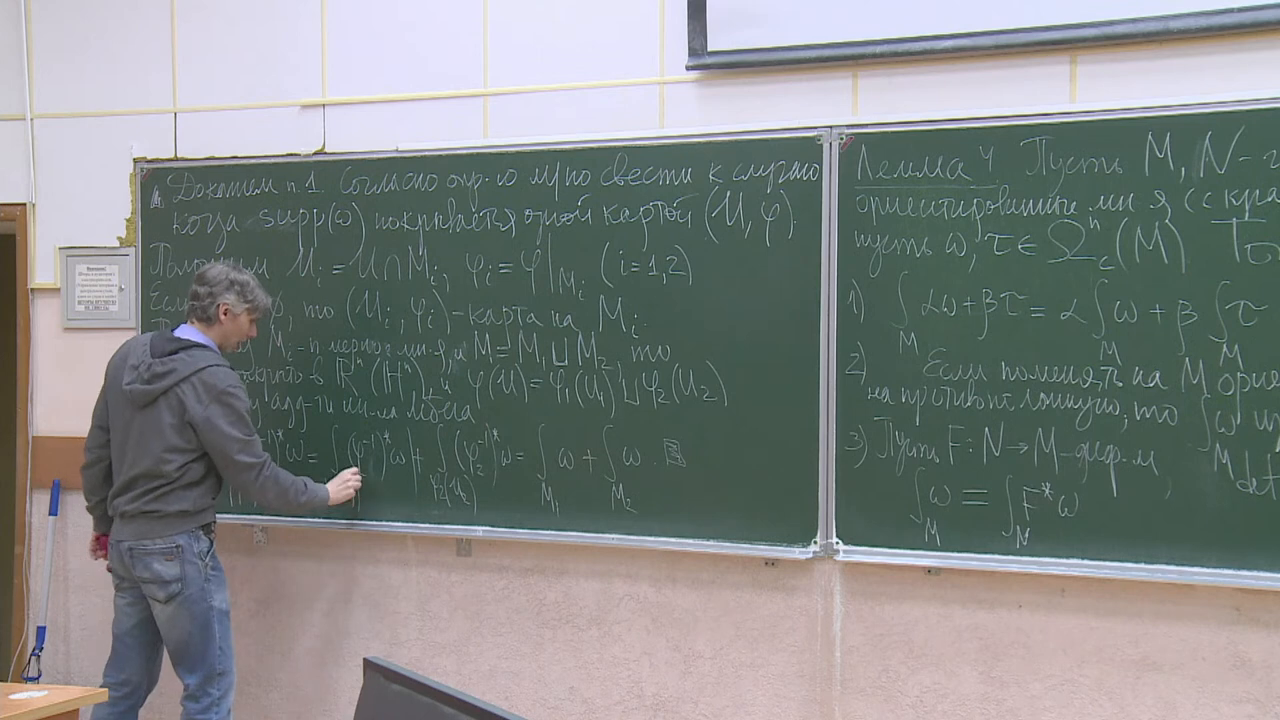
\includegraphics[width=0.3\textwidth]{images/kratnye_intergraly_left.png}
        \quad
        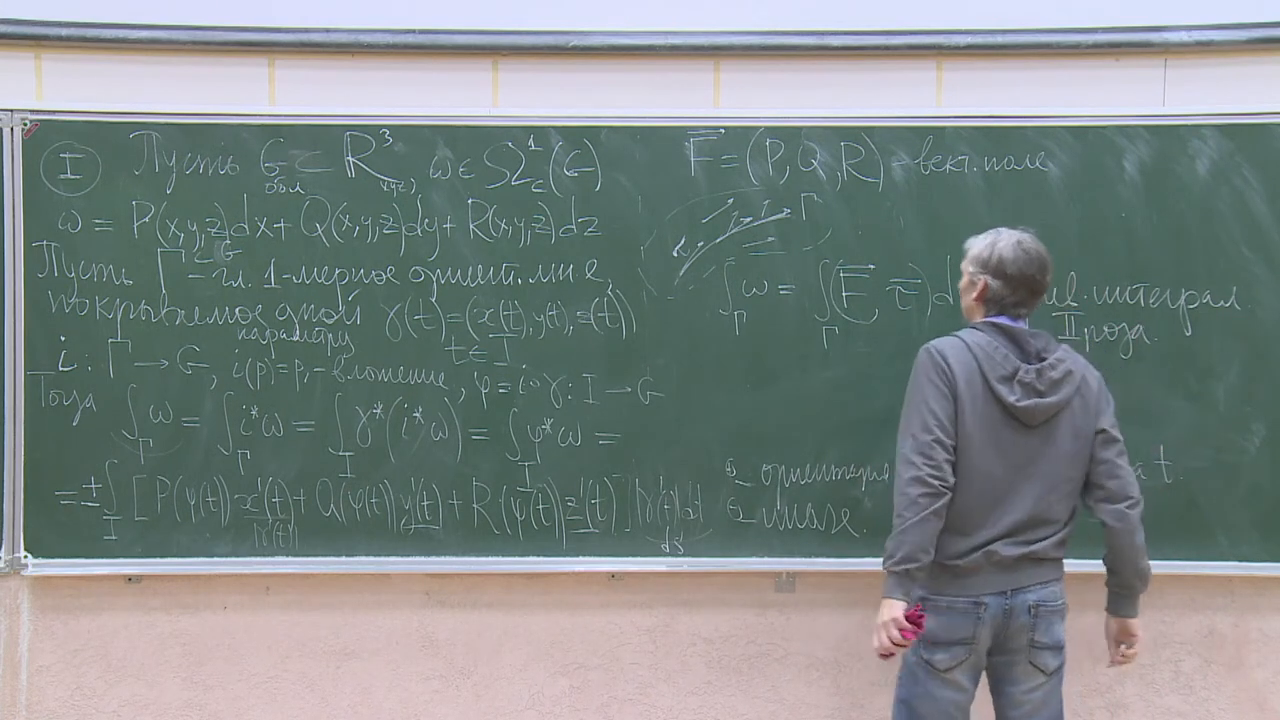
\includegraphics[width=0.3\textwidth]{images/kratnye_intergraly_center.png}
        \quad
        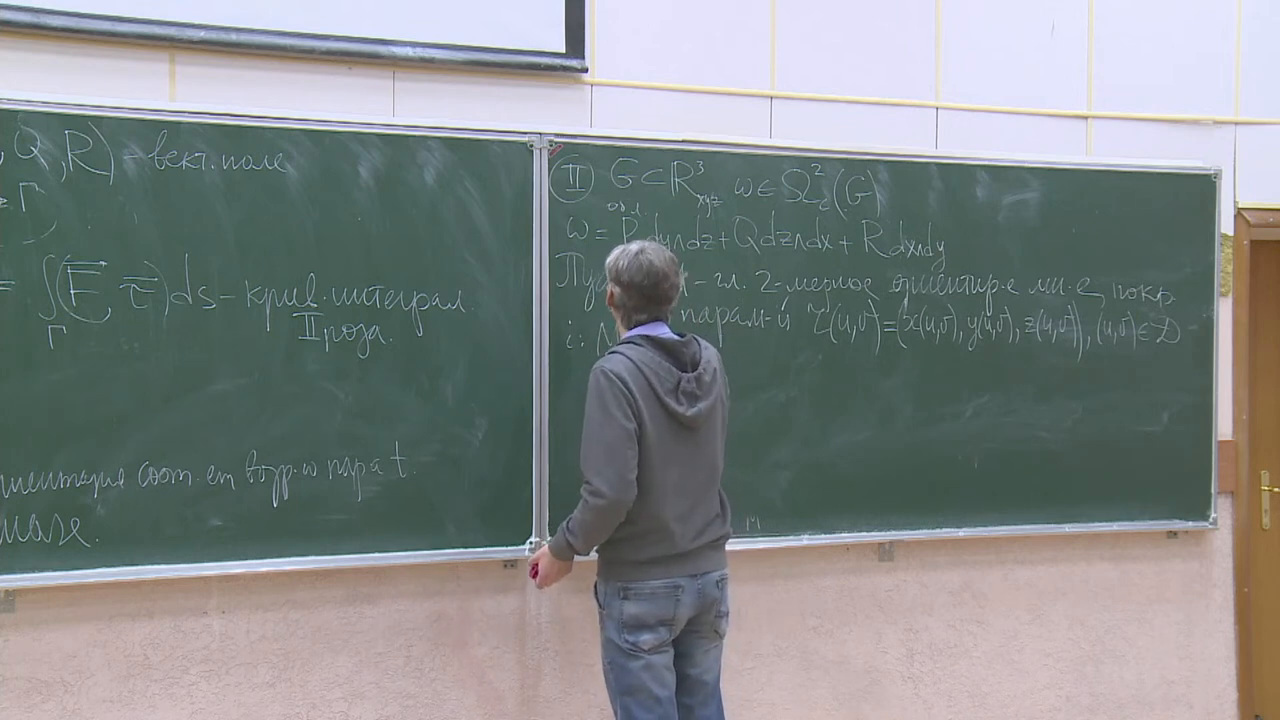
\includegraphics[width=0.3\textwidth]{images/kratnye_intergraly_right.png}
    \end{figure}
    \begin{figure}
        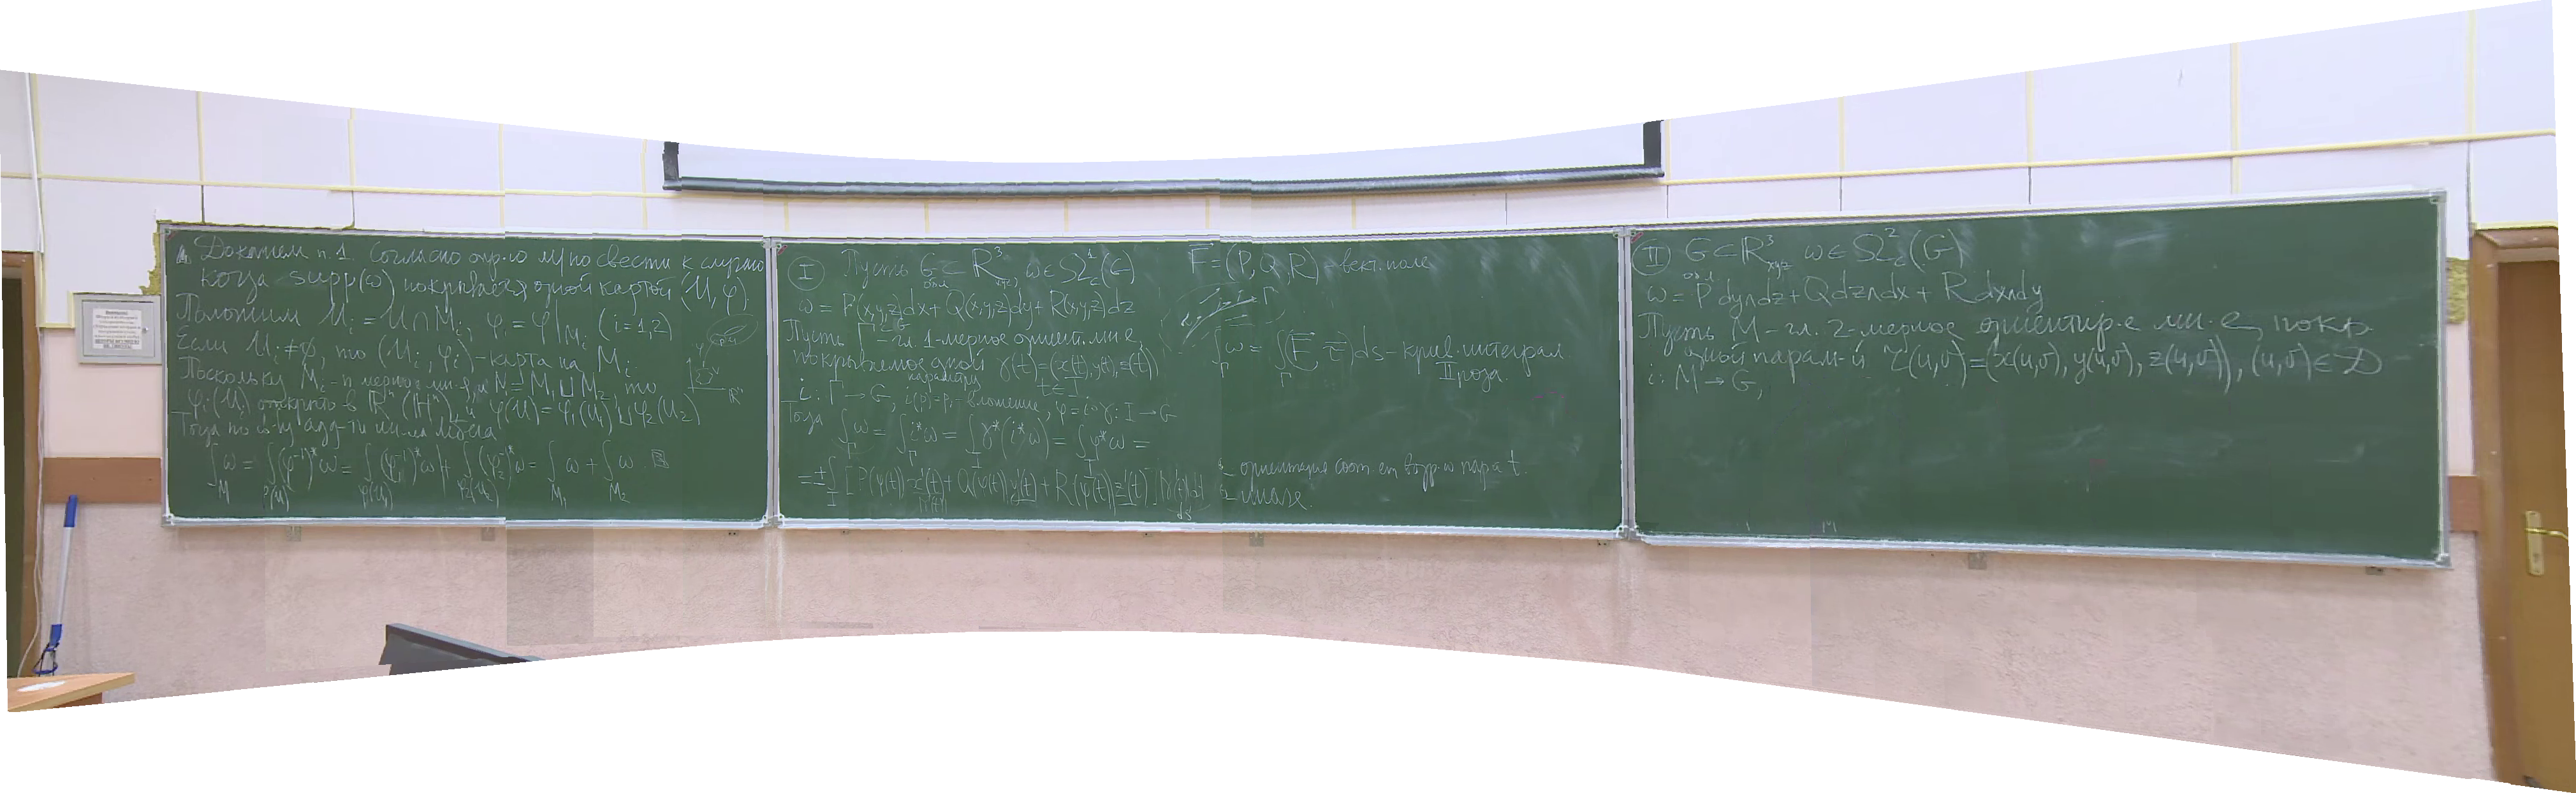
\includegraphics[width=0.8\textwidth]{images/kratnye_integraly_panorama.png}
    \end{figure}
\end{frame}

\begin{frame}
    \frametitle{Вступ}
    \textbf{Об'єкт дослідження}~---~відеозаписи лекцій. \\
    \textbf{Предмет дослідження}~---~автоматична обробка відеозаписів. \\ 
    \textbf{Метою роботи} є розробка інформаційної технології, що перетворює 
    відеозапис лекції у панорамні знімки без викладача. \\

    Дана інформаційна технологія повинна мати ряд властивостей:
    \begin{itemize}
        \item здатність працювати на звичайному смартфоні у режимі реального часу;
        \item можливість працювати з дошками різного кольору;
        \item можливість працювати з рухливою камерою;
        \item мінімальна кількість дефектів на слайдах,
            таких як наявність фрагментів викладача
            або видимі шви у місцях склейки кадрів.
    \end{itemize}
\end{frame}

\setbeamertemplate{section in toc}{\inserttocsectionnumber~\inserttocsection}
\pagenumbering{}
\begin{frame}
  \frametitle{Зміст}
    \tableofcontents
\end{frame}

\section{Процедура створення панорамних слайдів}
\begin{frame}
    \frametitle{Процедура створення панорамних слайдів}
    \usetikzlibrary{arrows,positioning,shapes}
    \begin{figure}[H]
        \begin{center}
            \begin{tikzpicture}[node distance=4mm, >=latex',
                    block/.style = {draw, rectangle, minimum height=10mm, minimum width=28mm,align=center},
                    rblock/.style = {draw, rectangle, rounded corners=0.5em},
                    tblock/.style = {draw, trapezium, minimum height=10mm,
                            trapezium left angle=75, trapezium right angle=105, align=center},
                ]
                \node [rblock]                           (video)        {Відео};
                \node [block, below=of video]            (mov_objects)  {Побудова маски\\
                    рухомих об'єктів або людини};
                \node [block, right=of mov_objects]      (pan)          {Побудова панорамами};
                \node [block, right=of pan]              (denoise)      {Зниження рівня\\ шуму};
                \node [rblock,above=of denoise]          (slides)       {Слайди};

                \path[draw,->] (video)         edge    (mov_objects)
                (mov_objects)   edge    (pan)
                (pan)           edge    (denoise)
                (denoise)       edge    (slides)
                ;
            \end{tikzpicture}
        \end{center}
    \end{figure}
\end{frame}

\section{Стабілізація відео}
\begin{frame}
  \frametitle{Стабілізація відео}

  Оскільки дошка~---~це плоска поверхня, ми можемо знайти матрицю гомографії між двома кадрами.
  Для цього використовуємо алгоритм SIFT та RANSAC.
  \begin{figure}[H]
    \centering
    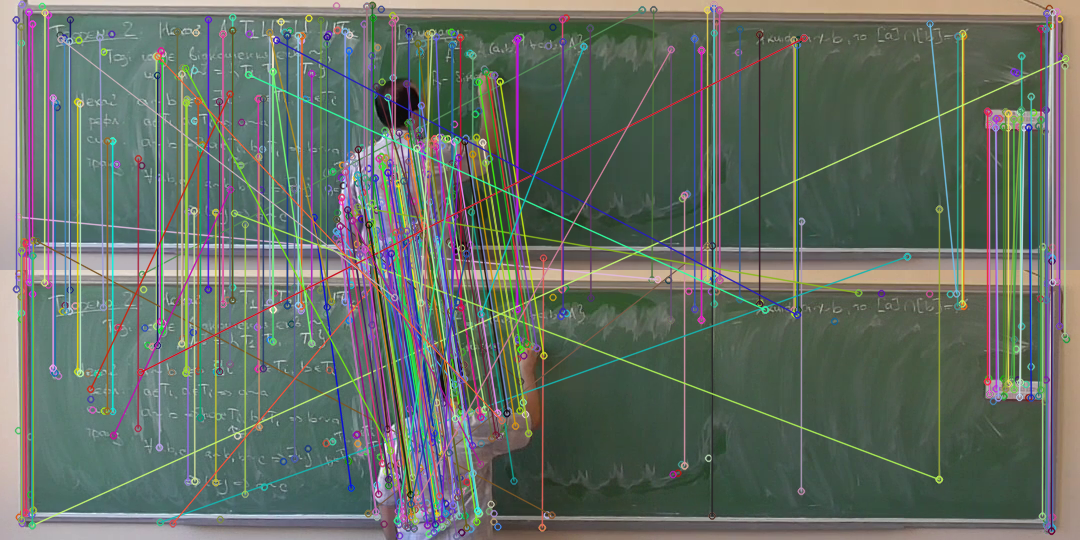
\includegraphics[width=0.55\textwidth]{images/matches_img}
    \caption{Кадри $F^i$ (верхній) та $F^{i+s}$ (нижній) із ключовими точками та лініями, \\
      які поєднують відповідні точки з відео
    }
  \end{figure}

\end{frame}

\section{Методи локалізації людини та рухомих об'єктів}
\begin{frame}
  \frametitle{Алгоритм Бойкова Колмогорова}

  Сформулюємо задачу максимального потоку
  \begin{equation*}
    \sum_{t \in N_s} f_{st} \rightarrow \max_{f: \tau \rightarrow R }
  \end{equation*}
  з обмеженнями
  \begin{equation*}
    \begin{gathered}
      \begin{cases}
        f_{tt^{'}} \leq  c_{tt^{'}},                                   & \forall tt^{'}  \in \tau ,         \\
        \sum_{p \in P_t} f_{pt} - \sum_{t^{'} \in N_t} f_{tt^{'}} = 0, & \forall t \in T \setminus \{s,e\}, \\
        \sum f_{tt^{'}} \geq 0,                                        & \forall tt^{'}  \in \tau.
      \end{cases}
    \end{gathered}
  \end{equation*}
  Це означає, що
  \begin{enumerate}
    \item потік має не перевищувати пропускну здатність для всіх ребер;
    \item сума потоків, що входять у вузол не повинна змінитись на виході;
    \item потік завжди додатній.
  \end{enumerate}
\end{frame}

%\section{Методи локалізації людини та рухомих об'єктів}
\begin{frame}
  \frametitle{Процес створення маски рухомих об'єктів алгоритмом Б-К}
  
  \begin{figure}[H]
	\centering
	\subfloat[Попередній кадр $F^i$]{
		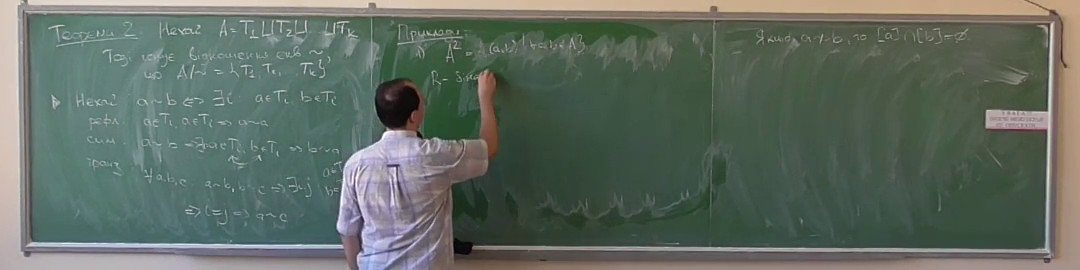
\includegraphics[width=0.45\textwidth]{images/prev_frame}
	}\\
	\subfloat[Поточний кадр $F^{i+s}$]{
		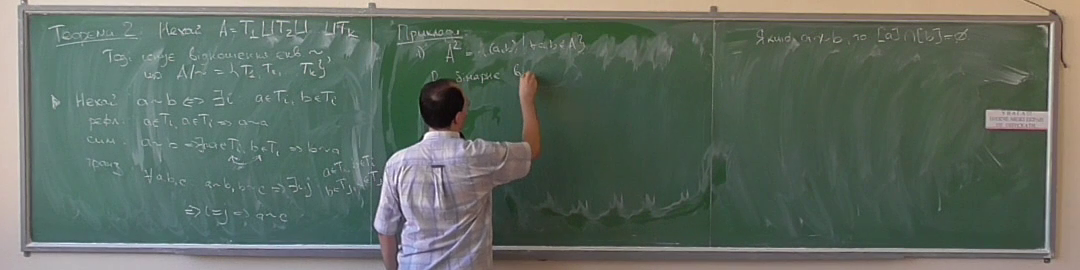
\includegraphics[width=0.45\textwidth]{images/next_frame}
	}\\
	\subfloat[Інвертована різниця $F^i$ і $F^{i+s}$]{
		
\includegraphics[width=0.45\textwidth]{images/inv_diff}
	}\\
	\subfloat[Маска рухомих об'єктів на кадрі $F^{i+s}$]{
		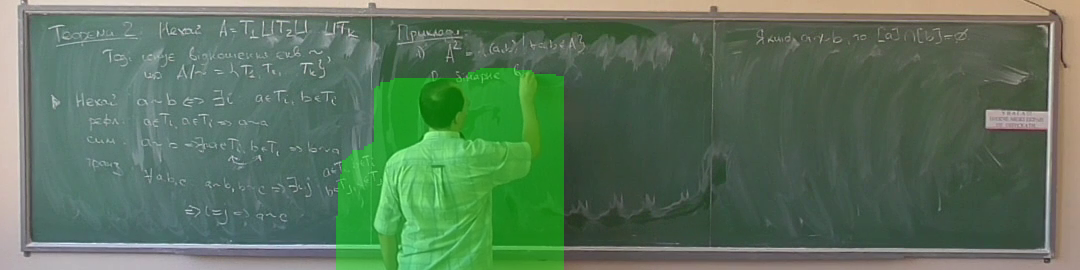
\includegraphics[width=0.45\textwidth]{images/next_with_mask}
	}
\end{figure}
\end{frame}



\end{document}
